\section{Introduction}

[In the previous chapter (DMFs) I show the evolution in dust masses assuming Galactic dust at all redshifts (i.e T=20K and beta=2), this chapter will tackle this assumption.]

\section{Dust Properties of DSFGs}

Interstellar dust plays a crucial role in the formation of galaxies as dust grains are the site of molecule formation like molecular hydrogen, $H_2$, the primary fuel for star formation (\citealt{Kennicutt_2012}). $H_2$ is the most abundant molecule in the Universe but is difficult to observe directly unless originating from energetic environments. Alternatives include observing less abundant molecules such as CO and using conversion factors to estimate the mass of molecular hydrogen, or observing dust emission to estimate dust masses (as in the previous chapter) and assuming gas-to-dust ratios (e.g. \citealt{Saintonge_2013}) to convert these into estimates for the total gas mass in high-redshift galaxies (e.g. \citealt{Magdis_2012}; \citealt{Eales_2012}; \citealt{Scoville_2014}; \citealt{Santini_2014}; \citealt{Genzel_2015}). Such studies have shown that galaxies at high redshift contain a higher fraction of gas than galaxies today (\citealt{Tacconi_2010}; \citealt{Scoville_2016}; \citealt{Scoville_2017}; \citealt{Millard_2020}), showing that direct observations of dust emission are useful in our understanding of how galaxies grow and evolve. It is important to note, however, that studies that make these links between dust emission and the evolution of galactic properties make the basic assumption that properties of the dust remain constant with redshift. In the following we investigate the possibility of evolution in dust itself by modelling the dust emission from a sample of high-redshift galaxies and measuring their dust properties over a large expanse of cosmic history.

Of particular importance to us is the dust emissivity spectral index, $\beta$, which controls the frequency dependence of the emissivity of dust grains per unit mass. By assuming, as is customary, that the optical depth of a galaxy can be approximated as a power law of the form $\tau \propto \nu^\beta$, we are implicity assuming that $\beta$ encodes within it information about the dust grain properties such as their chemical composition and their size and growth. The assumed value of $\beta$ for a galaxy can have significant consequences on the assumed absorption properties of the dust grains and consequently on fundamental properties of the ISM in the galaxy such as the total mass of dust (\citealt{Bianchi_2013}; \citealt{Clark_2016}).

Theoretical models for dust (e.g. \citealt{Draine_1984}; \citealt{Draine_2011}; \citealt{Kohler_2015}) predict $\beta$ values to range between approximately 1 -- 2 depending on the chemical composition of the dust grains. Adopting suitable fixed values of $\beta$ have been vital for estimates of the dust temperature and dust luminosity of galaxies in past studies, particularly for high-redshift sources that often lack constraints in the far-infrared (e.g. \todo[color=green]{Add references}). A nominal value of $\beta$ = 2 is common practice in this scenario as it mimics the emissivity of mixtures of amorphous silicates and graphites that well represent the optical properties of Galactic dust grains. However, recent studies have shown that the value of $\beta$ can take a wide variety of values among local galaxies and even among different regions within the same galaxy. For example, \citealt{Lamperti_2019} model the far-infrared dust SEDs of 192 nearby galaxies from the JCMT dust and gas In Nearby Galaxies Legacy Exploration (JINGLE) survey and observed a range of temperatures for the cold dust between 17 and 30\,K and dust emissivity spectral indices between 0.6 and 2.2. Within M31 (Andromeda) \citealt{Smith_2012}, \citealt{Draine_2014} and \citealt{Whitworth_2019} identified a decrease in $\beta$ with galactocentric radius, potentially a result of $\beta$ evolving to higher values when observed in denser regions of the ISM due to grain coagulation. A follow up study by \citealt{Athikkat-Eknath_2022} compared the average $\beta$ measured inside and outside molecular clouds within M31, and while there was no evidence to support the idea that $\beta$ varies due to dense molecular gas, the radial variation in $\beta$ remained present. At higher redshifts, where the far-infrared part of the spectrum is spatially unresolved, it is not possible to constrain the true value of a galaxy's $\beta$ but can be used to define an \textit{effective} $\beta$ value that represents the integrated dust properties over the whole galaxy. [...]\todo[color=orange]{Importance of having an effective $\beta$ value.}

\section{Obtaining Redshifts from Molecular Lines}

In order to study the evolution of the dust properties of DSFGs we require robust redshifts to place their formation in cosmic history and to determine accurate measurements of fundamental properties. Obtaining robust ages of galaxies in the form of spectroscopically determined redshifts is hampered by the poor spatial resolution of single-dish observations, which worsens with increasing redshift. While DSFGs can be discovered at far-infrared and sub-mm wavelengths to high redshifts directly from the photometry of the sub-mm source, selecting those with distinctly red sub-mm colours in the \textit{Herschel} bands (e.g. \citealt{Dowell_2014}; \citealt{Ivison_2016}; \citealt{Donevski_2018}; \citealt{Duivenvoorden_2018}), careful consideration of the selection wavelength is required to make optimal use of the negative K-correction. For example, the \textit{Herschel}-SPIRE bands increasingly probe the peak of the dust SED at higher redshifts, making them less sensitive to unlensed DSFGs beyond z $\sim$ 2 -- 3. Additionally, the dust-obscured nature of this population of galaxies makes the identification of counterparts at other wavelengths where spectroscopically determined reshifts are readily available more difficult, which is compounded by the poor resolution and source confusion in the sub-mm (see the Likelihod Ratio analysis of Chapter \ref{chapter:Data_Release_3} for an example).

A more reliable method for robust redshifts is to follow up single-dish observations with inteferometric measurements with interferometers such as the Atacama Large Millimeter/submillimeter Array (ALMA). An even more direct way of obtaining redshfits while observing sources in the sub-mm/mm wavebands is to observe molecular emission lines which can be directly associated with the sub-mm emission without the need for intermediary steps with high-resolution imaging. Recent advancements in the possible bandwidths of instruments like ALMA and the Northern Extended Millimetre Array (NOEMA) have allowed for the ability to detect spectral lines (typically from CO or [CII]) that emanate unambiguously from the sub-mm source. CO is the second most abundant molecule in the Universe after $H_2$ and has rotational transitions that produce some of the brightest lines in the millimeter spectrum. The brightness of the CO lines result from the abundance of CO, the low excitation energy of the transitions and the wavelengths at which they occur coinciding with regions of the spectrum with high atmospheric transmission probed by ALMA. A secondary advantage of using molecular emission to determine spectroscopic redshifts is that they are independent of the photometry used to describe the dust SED and are therefore less prone to bias. In Figure \ref{fig:redshift_ladder} I show the coverage of CO line transitions as functions of the redshift and observed wavelength. We see that at [...] wavelengths, there is a non-uniform coverage of CO transitions, meaning that sources believed to be at a particular redshift may have multiple line detections, allowing for unambiguous constraints on the redshift of the galaxy, single line detections, which allows for some abiguity to the redshift solution, or no line detections. In the regions where no CO lines can be detected by a particular instrument, "redshift deserts" appear as breaks in the redshift distribution of galaxies.


\begin{figure}
	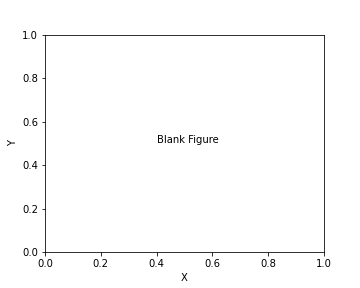
\includegraphics[width=\columnwidth]{Figures/blank_figure.png}
	\caption{Caption}
	\label{fig:redshift_ladder}
\end{figure}

\section{Sample Creation}
\subsection{South Pole Telescope DSFGs}
\subsection{The HerBS Sample}
\section{Far-Infrared and Sub-mm Colours}
\section{The Modified Blackbody Model}
\section{SED Fitting of DSFGs}
\subsection{Posterior Distributions}
\subsection{The Dust Emissivity Spectral Index - Dust Temperature Degeneracy}
\section{Accuracy of Dust Parameters}
\subsection{Simulations of SPT and HerBS Sources}
\subsection{Results of Simulations}
\section{The Properties of Dust in DSFGs}
\subsection{The Diversity of Dust Emissivity Spectral Indices and their Evolution with Redshift}
\subsection{The Diversity of Dust Temperatures and their Evolution with Redshift}
\subsection{Implications of Evolving Dust Properties between 2 < z < 6}
\section{Conclusions}

\listoftodos